\chapter{Clustering}

Clustering is a prime example of a problem typically associated with unsupervised learning.\footnote{In this work, both unsupervised and supervised approaches to clustering are explored.} \cite{xu_comprehensive_2015} even call clustering the most important question of unsupervised learning. The task is one of grouping objects into \name{clusters} such that the objects in any particular cluster are in some sense more similar to each other that to the objects from other clusters. Alternatively, the problem can be formulated as one finding a similarity measure on the object space such that the objects deemed to be similar actually are under the measure. Oftentimes, such a similarity measure is based on some distance function such as the Euclidean, Manhattan, Cosine, Minkowski or Mahalanobis (see \cite{mahalanobis_generalised_1936}) distance.

\section{Definition of clustering}
So far, the definition of terms such as "cluster" or "similar" has been left intuitive and vague. The reason for that is that there is no universal definition of what a cluster is. \cite{estivill-castro_why_2002} argues that there even should not be a universal definition as the clusters are, in a large part, on the eye of the beholder. Notwithstanding that, there is at least an informal definition provided by \cite{jain_algorithms_1988}:

\begin{enumerate}
	\item A cluster is a set of entities which are \textit{alike} and entities from different clusters are not alike.
	\item A cluster is an aggregation of points in the test space such that the \textit{distance} between any two points in the cluster is less than the distance between any point in the cluster and any point not in it.
	\item Cluster may be described as connected regions of a multi-dimensional space containing a relatively \textit{high density} of points, separated from other such regions by a region containing a relatively low density of points.
\end{enumerate}

Even with that definition, it is sometimes not clear what constitutes a cluster without some additional context. \cite{jain_algorithms_1988} presents figure \ref{fig:cluster-ambiguity} as an example.

\begin{figure}[ht]
	\centering
	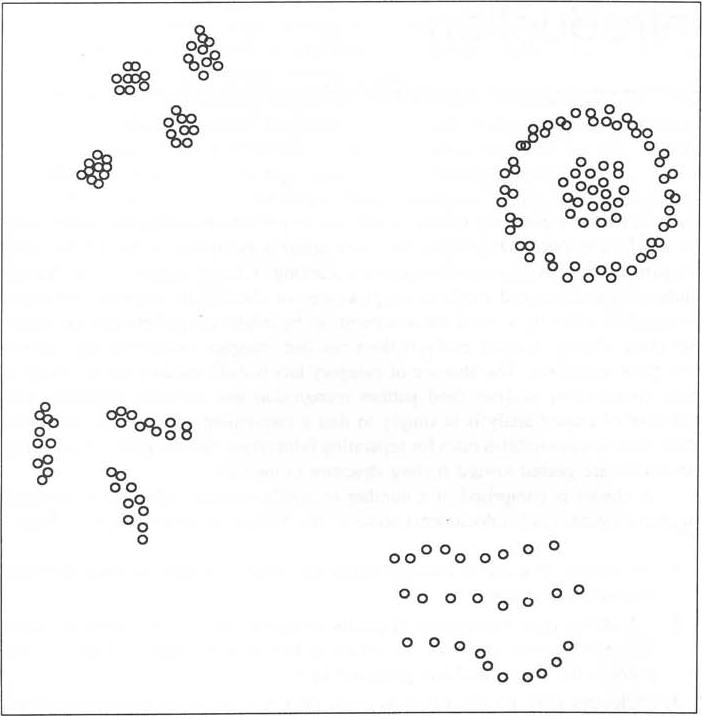
\includegraphics[width=0.9\textwidth]{images/cluster-ambiguity.png}
	\caption{An example of the ambiguity of clusters from \cite{jain_algorithms_1988}. At the global level, there are four clusters in the scatter plot. At a local level, or a lower similarity threshold, twelve clusters can be recognised however.}\label{fig:cluster-ambiguity}
\end{figure}

\cite{xu_comprehensive_2015} offers a comprehensive survey of different distance functions, similarity functions, evaluation indicators and clustering algorithms.

\section{Application to MIL}\label{sec:mil-clustering}

In the previous section it has been described what is a clustering. The link between clustering and multi-instance learning is, however, yet to be shown. In this section, the application of clustering to MIL is described.

The problem at hand is not one of clustering ordinary number vectors in a linear space. Instead, a clustering of objects represented by bags is explored, as that is the problem solved for datasets introduced later in chapters \ref{chap:toy-dataset} and \ref{chap:cisco-dataset}. While \cite{wang_solving_2000} present a clustering of bags using a modified Hausdorff distance on bags, this approach was not chosen in this work. Among the main reasons for this choice is the prohibitively high computational complexity of bag-space paradigm approaches on large datasets and the opportunity to utilize the representations previously introduced for the particular datasets in \cite{dedic_hierarchicke_2017}.

An approach based on the embedded-space paradigm (see section \ref{sec:embedded-space-paradigm}) for MIL was chosen. In order to utilize the structure of the data, a MIL model is used to represent each bag in the latent space \( \bar{\mathspace{X}} \). This presents the issue of how to train the embedding function \( \phi \) -- MIL as presented in chapter \ref{chap:MIL} is a supervised algorithm, whereas clustering is a typically unsupervised problem.

The embedding function \( \phi \) from section \ref{sec:embedded-space-paradigm} is actually of the form
\[ \phi = \phi \left( B, \mathvec{\theta} \right) \qquad \text{where} \quad B \in \mathspace{B} \]
where \( \mathvec{\theta} \) are the parameters of the embedding, typically learned during the training phase. In the context of clustering, these parameters still need to be learned over the training phase somehow. This in and of itself presents another challenge though -- off-the-shelf algorithms typically work in some kind of constant Hilbert space, whereas in this example, the latent space needs to change over the learning period. As is the case for MIL itself, end-to-end learning was chosen as an approach to solve both of these problems. A clustering-loss function \( L_C \) is chosen such that
\[ L_C: \mathcal{P}^M \left( \bar{\mathspace{X}} \right) \to \mathfield{R} \]
Given such clustering-loss function, an actual loss for the embedding model \( \phi \) and its parameters \( \mathvec{\theta} \) can be computed as
\[ L \left( \phi, \mathvec{\theta} \right) = L_C \left( \left\{ \phi \left( B, \mathvec{\theta} \right) \middle| B \in \mathspace{B} \right\} \right) \]
If the cluster-loss \( L_C \) is chosen correctly, minimizing \( L \) over the learning period will yield a latent space \( \bar{\mathspace{X}} \) in which the bags are already naturally clustered according to the design of the cluster-loss function. Applying any off-the-shelf clustering algorithm on \( \bar{\mathspace{X}} \) will then give good results. How to choose the cluster-loss function \( L_C \) is the focus of chapter \ref{chap:clustering-metric}.

\section{Clustering evaluation metrics}

\cite{xu_comprehensive_2015} present different clustering evaluation indicators. In this work, several indicators are used. The primary indicators are based on the Silhouette coefficient, the secondary ones on the kNN algorithm (see \cite{dasarathy_nearest_1991}). The indicators are somewhat different to the ones traditionally used in evaluating clustering methods as all the datasets used in this work are originally classification datasets and therefore have classes available. Each class can then be viewed as a cluster target and the learned clustering evaluated against these targets.

The first two indicators measure the \name{homogeneity} and \name{separation} of clusters (see \cite{everitt_cluster_2001}). To measure the homogeneity of a cluster, the average distance between items in a cluster is measured and averaged over all clusters, giving the following indicator for items \( x_j \) in clusters \( C_i \) (defined by the classes in the data):
\[ \mathrm{homo} \left( C_1, \dots, C_n \right) = \frac{1}{n} \sum_{i = 1}^n \frac{1}{\left\lvert C_i \right\rvert} \sum_{\substack{x_j, x_k \in C_i \\ x_j \neq x_k}} \left\lVert x_j - x_k \right\rVert \]
To make this indicator computationally less complex, it can be simplified by extracting the centre \( \mu \) of the cluster:
\[ \mu \left( C_i \right) = \frac{1}{\left\lvert C_i \right\rvert} \sum_{x_j \in C_i} x_j \]
\[ \mathrm{homo} \left( C_1, \dots, C_n \right) = \frac{1}{n} \sum_{i = 1}^n \sum_{x_j \in C_i} \left\lVert x_j - \mu \left( C_i \right) \right\rVert \]

To measure the separation of clusters, the average distance between cluster centres was taken:
\[ \mathrm{sep} \left( C_1, \dots, C_n \right) = \frac{2}{n \left( n - 1 \right)} \sum_{\substack{i, j \in \hat{n} \\ i < j }} \left\lVert \mu \left( C_i \right) - \mu \left( C_j \right) \right\rVert \]

The final primary indicator is akin to a simplified Silhouette coefficient:
\[ \mathrm{ratio} \left( C_1, \dots, C_n \right) = \frac{\mathrm{sep} \left( C_1, \dots, C_n \right)}{\mathrm{homo} \left( C_1, \dots, C_n \right)} \]

For the secondary indicators, the kNN algorithm is used and its accuracy (i.e. the fraction of correctly classified samples) measured. The kNN algorithm was seeded with the training data and its accuracy assessed on the testing data. This was done over the learning period, giving the first indicator. Secondly, on the final model, the kNN classifier has been seeded with different amount of data and its performance measured. This gives a view into the robustness of the clustering, as high-quality embeddings would need only a small amount of seed data points to reach relatively high accuracy.

\todo{Present K-means, kNN and self-tuning spectral clustering?}
